%========ANÁLISIS DEL MODULO DE COMUNICACIÓN=======

\subsection{Sistema operativo móvil}
Los sistemas operativos para teléfonos inteligentes o sistemas operativos móviles son sistemas operativos que operan teléfonos inteligentes, PDA, tabletas y otros dispositivos móviles. Un sistema operativo permite que estos dispositivos ejecuten aplicaciones y programas, por lo tanto, llevan funciones avanzadas a dispositivos móviles que anteriormente estaban restringidos a computadoras de escritorio. \\

En la figura \ref{fig:grafica_mercadoOS} se muestra una gráfica que indica la participación de mercado global del sistema operativo móvil, en términos de ventas a usuarios finales, de 2009 a 2018. En el segundo trimestre de 2018, el 88\% de los teléfonos celulares vendidos a usuarios finales eran teléfonos con el sistema operativo Android \cite{mercadoOS}. \\

\begin{figure}[htbp!]
	\centering
	\fbox{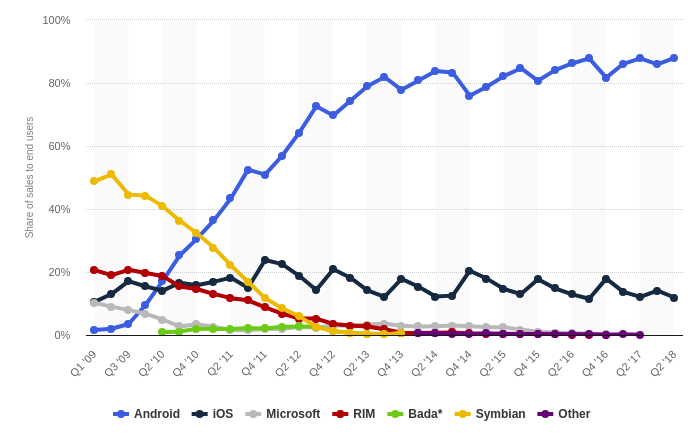
\includegraphics[width=0.9\textwidth]{Analisis/imagenes/mercadoOS.png}}
	\caption{Sistemas operativos móviles en el mercado global. Statista (2018).}
	\label{fig:grafica_mercadoOS}
\end{figure}

A pesar de existir varios sistemas operativos móviles como: Microsoft, Symbian, RIM, Android, iOS, entre otros, son dos los que actualmente abarcan casi la totalidad del mercado: Android e iOS, por lo que para el desarrollo de la aplicación móvil únicamente se considerarán éstos dos. \\

\textbf{Android} es un sistema operativo móvil desarrollado por Google. Está basado en Linux y está enfocado para ser utilizado en dispositivos móviles como smartphones, tablets, Google TV y otros dispositivos \cite{android}, que ofrece un completo framework de aplicaciones que te permite crear apps y juegos innovadores para dispositivos móviles en un entorno de lenguaje Java \cite{androidJava}. \\

\textbf{iOS} es un sistema operativo móvil desarrollado por Apple que se ejecuta en los dispositivos iPhone, iPad, iPod Touch y otros dispositivos de Apple \cite{nations2018iOS}. Para desarrollar aplicaciones de iOS, Apple ofrece Swift, que es un lenguaje de programación poderoso e intuitivo \cite{swift}. \\

Ambos sistemas operativos tienen características comunes importantes para el desarrollo de la aplicación móvil, tal como se muestra en la tabla \ref{analisis:caracteristicasOS}. 

\begin{table}[htbp!]
	\begin{center}
		\scalebox{0.70}[0.80]{
		\begin{tabular}{|c|c|}
			\hline
			%			\rowcolor{colorSecundario}
			%			\color{green}
			\thead{Caracterísitca}&\thead{Descripción}\\
			\hline
			\hline
			Conectividad & Soportan múltiples tecnologías de comunicación, incluyendo GSM.\\
			\hline
			Almacenamiento & Soportan el manejo de gestores de bases de datos como SQLite.\\
			\hline
			Mensajería & Están disponibles las formas de mensajería SMS y MMS.\\
			\hline
			Multitarea & Está disponible la multitarea de aplicaciones, permitiendo la ejecución de varias aplicaciones simultáneamente.\\
			\hline
		\end{tabular}
		}
		\caption{Características comunes de los sistemas operativos Android e iOS. Adaptado de Shailendra (2015).}
		\label{analisis:caracteristicasOS}
	\end{center}
\end{table}
	
En la figura \ref{fig:mapaOS} se muestra la preferencia de los países por cierto sistema operativo, ya sea Android o iOS. Se puede observar que el sistema operativo dominante en el mercado mexicano es Android. \\

\begin{figure}[htbp!]
	\centering
	\fbox{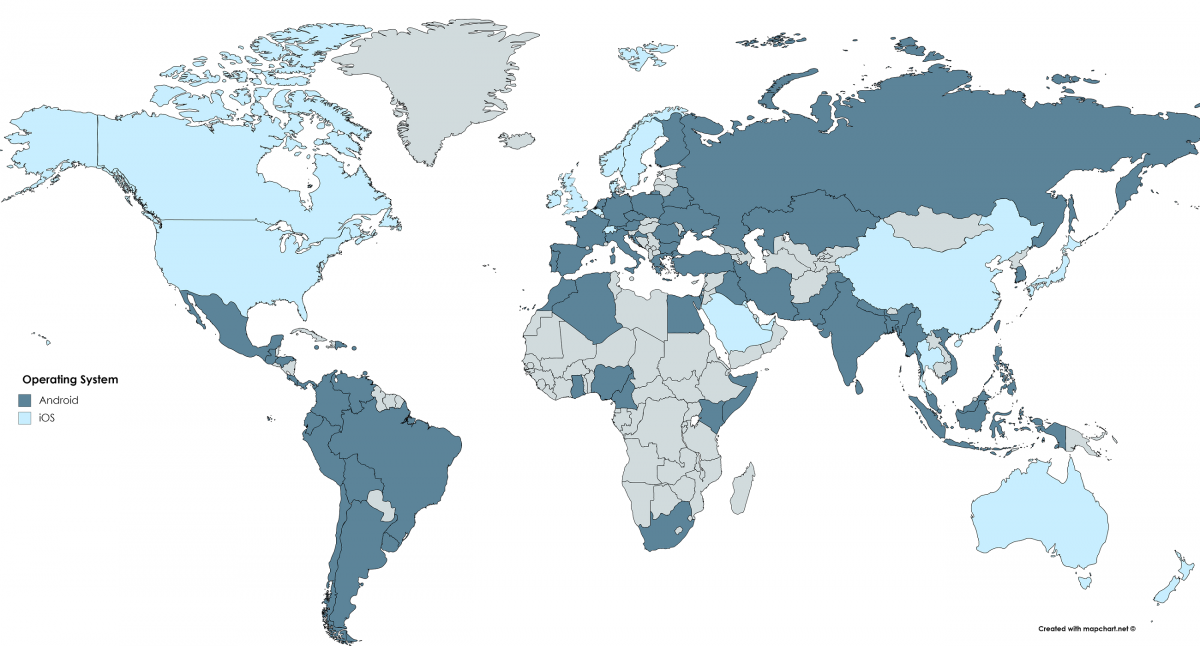
\includegraphics[width=0.9\textwidth]{Analisis/imagenes/mapaOS.png}}
	\caption{Mapa de popularidad de sistemas operativos Android e iOS. DeviceAtlas (2018).}
	\label{fig:mapaOS}
\end{figure}

En la figura \ref{fig:mercadoMexico} se muestra el porcentaje de dispositivos vendidos con sistema operativo Android (81.45\%) e iOS (17.34\%) en México, indicando una gran diferencia entre la cantidad de dispositivos con estos sistemas operativos vendidos entre octubre de 2017 y septiembre de 2018. \\

\begin{figure}[htbp!]
	\centering
	\fbox{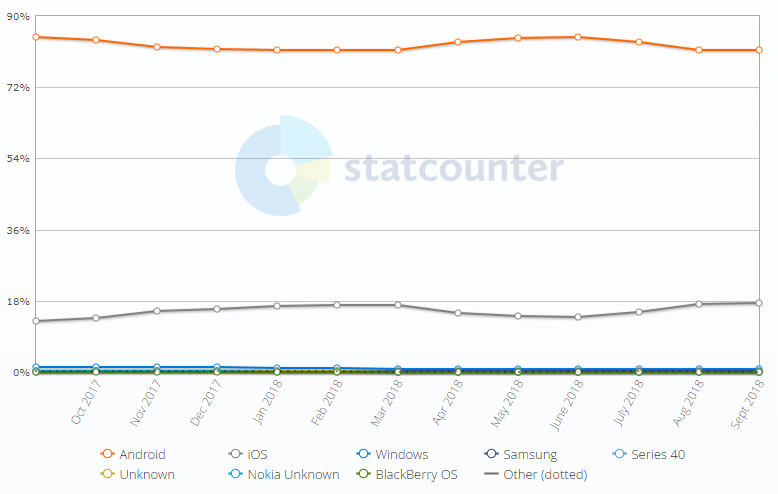
\includegraphics[width=0.9\textwidth]{Analisis/imagenes/mercadoMexico.png}}
	\caption{Sistemas operativos móviles en México. Statcounter (2018).}
	\label{fig:mercadoMexico}
\end{figure}

Debido a la popularidad del sistema operativo Android en México, se decidió desarrollar la aplicación para este sistema operativo y así lograr que pueda ser utilizado por un mayor número de personas. En la figura \ref{fig:versionesAndroid}. se muestra el porcentaje de dispositivos que  usan una versión determinada de la plataforma Android. \\

\begin{figure}[htbp!]
	\centering
	\fbox{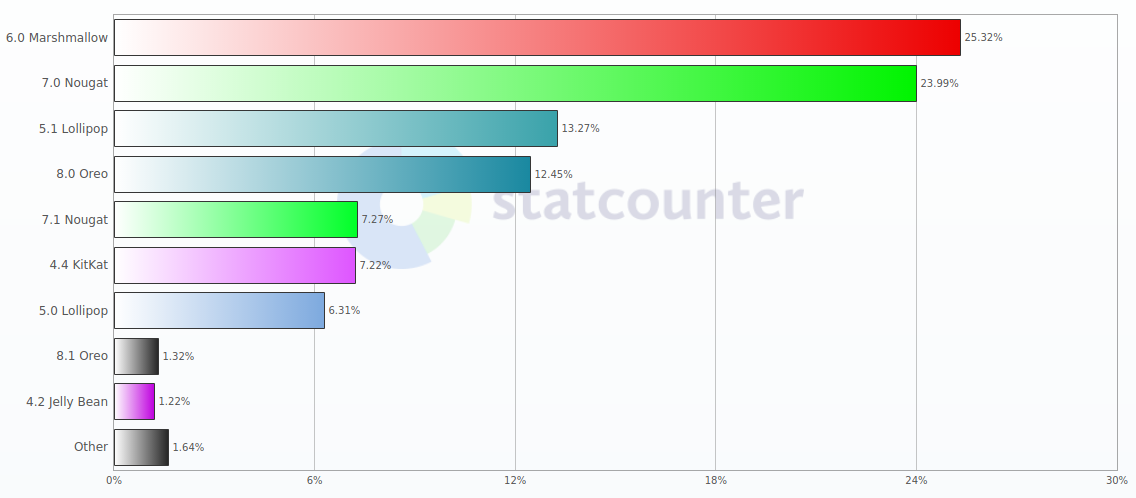
\includegraphics[width=0.9\textwidth]{Analisis/imagenes/versionesAndroid.png}}
	\caption{Versiones de Android utilizadas en México. Statcounter (2018).}
	\label{fig:versionesAndroid}
\end{figure}

Por lo tanto la aplicación móvil será desarrollada para el sistema operativo Android y se buscará que sea compatible con la versión más reciente, Oreo 8.1, y las versiones Nougat 7.0 y 7.1, y Marshmallow 6.0 con la finalidad de que sea compatible con el mayor porcentaje de dispositivos y poder realizar pruebas con algún dispositivo físico más fácilmente. \\

\clearpage